%%% AgriHome — Project Charter (updated release, Summer 2026)
%%% Structure aligned with CSE 4316 / UTA senior design charter template

\documentclass[11pt,letterpaper]{article}
\usepackage[margin=1.0in]{geometry}
\usepackage[T1]{fontenc}
\usepackage[utf8]{inputenc}
\usepackage{array}
\usepackage{booktabs}
\usepackage{longtable}
\usepackage{xcolor}
\usepackage{graphicx}
\usepackage{float}
\usepackage[hidelinks]{hyperref}
\usepackage{fancyhdr}
\usepackage{lastpage}
\usepackage{tikz}
\usetikzlibrary{arrows.meta,positioning,fit,calc}

\graphicspath{{images/}}

\definecolor{accentcolor}{rgb}{0.0,0.0,0.5}
\definecolor{leafgreen}{RGB}{61,159,108}

\newcommand{\teamname}{AgriHome}
\newcommand{\coursename}{CSE 4316 / CSE 4317: Senior Design}
\newcommand{\semester}{Summer 2026}
\newcommand{\docname}{Project Charter}
\newcommand{\department}{Department of Computer Science \& Engineering}
\newcommand{\university}{The University of Texas at Arlington}
\newcommand{\authors}{%
  GOVINDA AWASTHI\\
  LAXMAN BHUSHAL\\
  THUC DANG\\
  SAGAR KHADKA\\
  MUHAMMAD SAAD MEMON\\
  ALEX TABLIZO\\
  NATHAN NGUYEN TRAN}

\pagestyle{fancy}
\lhead{}
\chead{}
\rhead{}
\lfoot{\footnotesize \teamname\ - \semester}
\cfoot{}
\rfoot{\footnotesize page \thepage\ of \pageref{LastPage}}
\renewcommand{\headrulewidth}{0.0pt}
\renewcommand{\footrulewidth}{0.4pt}

\begin{document}

%%% Cover sheet
{\centering \huge \color{accentcolor} \scshape \textbf{\department \\ \university} \par}
\vspace{0.65in}
{\centering \huge \color{accentcolor} \scshape \textbf{\docname \\ \coursename \\ \semester} \par}
\vspace{0.4in}
\begin{center}
	
\includegraphics[width=0.52\textwidth]{agrihome-logo}\\[0.55em]
	{\small\slshape AgriHome project logo: leaf and camera lens motif for vision-based agricultural monitoring.}
\end{center}
\vspace{0.45in}
{\centering \huge \color{accentcolor} \scshape \textbf{\teamname} \par}
\vspace{0.25in}
{\centering \large \scshape \textbf{\authors} \par}
\newpage

\section*{Revision History}
\begin{center}
\begin{tabular}{@{}llll@{}}
\toprule
\textbf{Revision} & \textbf{Date} & \textbf{Author(s)} & \textbf{Description} \\
\midrule
0.1 & 02.18.2026 & MM & Document creation \\
0.2 & 02.2026 & Team & Complete draft \\
0.3 & 02.2026 & Team & Release candidate 1 \\
1.0 & 03.2026 & Team & Official release \\
1.1 & 03.2026 & Team & Customer change requests \\
2.0 & 07.23.2026 & Team & Summer update: Pi/Moonraker edge + Vision Console \\
2.1 & 07.28.2026 & Team & Klipper edge: Agri-Home/klipper + fswebcam; klipper\_url \\
\bottomrule
\end{tabular}
\end{center}
\newpage

\tableofcontents
\newpage
\listoffigures
\listoftables
\newpage

\section{Problem Statement}
Plant health management remains a significant challenge for farmers, gardeners, and greenhouse
operators. Plant disease often goes undetected in early stages as symptoms may be unseen, mistaken
for deficiencies, or environmental stress. Accurate diagnosis usually requires specialized knowledge,
and many individuals cannot identify plant health issues efficiently. Incorrect identification may
result in infection spread, reduced crop yield, and financial loss.

There is a need for a reliable system that provides early detection and continuous observation of plant
health. Accurate disease identification would allow users to respond more effectively, encourage a
healthier growing environment, and minimize crop damage. Addressing this issue improves plant
health management while supporting informed decision-making in both large-scale facilities and
small-scale home gardening environments.

Through Summer 2026, AgriHome has narrowed the practical gap between \emph{manual inspection}
and \emph{always-on monitoring} by pairing a Vision Console web application with edge hardware
(Raspberry Pi capture rigs) that can register themselves, report online status, and deliver tray imagery
into a durable PostgreSQL-backed store for operator review and optional computer-vision analysis.

\section{Methodology}
AgriHome is a plant-health monitoring system built around continuous observation and early issue
detection. The system captures plant imagery on a regular basis---via operator-initiated Take Picture
commands, capture schedules destined for \texttt{raspberry-pi-edge}, or manual uploads---and analyzes
images to detect irregularities when a computer-vision backend is configured.

The implemented stack through Summer 2026 includes:
\begin{itemize}
  \item \textbf{Vision Console} --- a Next.js App Router progressive web application with responsive
        desktop sidebar and mobile bottom navigation.
  \item \textbf{Identity} --- Firebase Authentication (email/password and Google) with server-verified
        session cookies for protected routes and APIs.
  \item \textbf{Data plane} --- PostgreSQL as the system of record for trays, plants, captures, schedules,
        edge devices, commands, and monitoring events; local file storage under configurable
        \texttt{STORAGE\_*} roots served via \texttt{/api/files/...}.
  \item \textbf{Edge capture} --- Raspberry Pi devices running
        \href{https://github.com/Agri-Home/klipper}{Agri-Home/klipper} (camera macros /
        \texttt{fswebcam} via \texttt{save\_image.sh}) plus the \texttt{agrihome\_agent} package
        (still hosted under the Agri-Home/moonraker repo companion): auto-provisioning, heartbeat,
        multipart ingest, and command claim/complete for capture workflows.
  \item \textbf{Optional CV} --- a \texttt{cv-backend} species/leaf classifier reached via
        \texttt{CV\_SPECIES\_INFERENCE\_URL}, with optional auto disease detection after Pi capture when
        enabled.
\end{itemize}

Using image recognition and machine learning when available, the system evaluates plant conditions
and surfaces potential issues based on visual symptoms. When irregularities are detected, the Console
presents status, reports, and monitoring events so operators can act before conditions worsen. The
monitoring process is continuous rather than one-off manual inspection.

\section{Value Proposition}
AgriHome offers value by combining accessible computer vision with an operable edge-to-cloud
workflow that greenhouse and lab users can run without becoming ML or embedded specialists.

For agricultural stakeholders, early identification of plant health issues reduces financial risk and
improves crop quality. For university and academic stakeholders, the project integrates computer
science, embedded systems, and agricultural applications, strengthening applied research and
demonstration capacity. The Summer 2026 edge integration specifically reduces operator toil:
devices self-provision into trays, report heartbeat/online status, and deliver frames through a secure
device API key path rather than ad-hoc file transfer.

By investing funding, time, and expertise, stakeholders support innovation in sustainable agriculture,
advance applied research, and contribute to a solution with meaningful economic and environmental
impact.

\section{High-Level Requirements}
The following capabilities define Summer~2026 scope at charter level (detailed in the SRS):

\begin{itemize}
  \item \textbf{Vision Console} --- authenticated Progressive Web App (Next.js App Router) for
        dashboard, trays, plants, Devices list, and tray Raspberry~Pi panel actions.
  \item \textbf{Identity} --- Firebase Authentication with server-verified session cookies for human
        operators; device identity remains separate from Firebase users.
  \item \textbf{Persistence} --- PostgreSQL as system of record for trays, plants, captures, schedules,
        \texttt{edge\_devices}, device commands, and monitoring events; image files under
        \texttt{STORAGE\_*} served via \texttt{/api/files/...}.
  \item \textbf{Edge provisioning} --- Raspberry~Pi agents register with CPU serial, MAC, hostname,
        and \texttt{DEVICE\_PROVISIONING\_SECRET}; AgriHome creates an \texttt{edge\_devices} row,
        hashed API key (plaintext shown once), and a linked tray.
  \item \textbf{Heartbeat \& commands} --- agents report online status and claim pending commands
        (including \texttt{capture\_now}) on a short interval.
  \item \textbf{Take Picture} --- primary path queues agent capture (\texttt{fswebcam} /
        \texttt{camera-macros/save\_image.sh} on Agri-Home/klipper); optional server-side HTTP
        streamer still when stored \texttt{klipper\_url} is reachable, then multipart ingest.
  \item \textbf{Ingest \& attach} --- authenticated multipart upload creates \texttt{camera\_captures};
        plants may auto-attach to the linked tray; optional disease/species detection after Pi capture
        when \texttt{cv-backend} / \texttt{DEVICE\_AUTO\_VISION\_ON\_INGEST} is configured.
  \item \textbf{Connectivity} --- Pi agents reach the AgriHome cloud URL over the network (LAN or
        Cloudflare tunnel / public HTTPS as needed); optional \texttt{klipper\_url} streamer bases may
        use a tunnel when the AgriHome host cannot reach the Pi LAN for server-side stills.
  \item \textbf{Security} --- rotatable provisioning secret, hashed device keys, revoke/rotate, ingest
        rate limits and size caps (see \texttt{docs/ops/EDGE\_DEVICE\_SECURITY.md}).
\end{itemize}

\section{Development Milestones}
\begin{itemize}
  \item Project Charter first draft --- February 2026
  \item System Requirements Specification --- March 2026
  \item Architectural Design Specification --- April 2026
  \item Demonstration of AI detection and test rig --- April 2026
  \item Vision Console (Next.js) + PostgreSQL + Firebase auth baseline --- Spring 2026
  \item \texttt{cv-backend} species classifier training/serving integration --- Spring--Summer 2026
  \item \textbf{Hardware \& Software Integration (Pi) sprint} --- Summer 2026
        (auto-provision \texttt{edge\_devices}, device API keys, heartbeat, Take Picture, multipart
        ingest, optional disease detection after Pi capture, plant auto-attach to tray)
  \item Edge agent reference package (\texttt{agrihome\_agent}; Klipper/fswebcam capture) --- Summer 2026
  \item Detailed Design Specification (CSE~4317) --- Summer 2026
  \item Demonstration of AI improvements and User Interface --- TBA
  \item Demonstration of web server, edge, and AI integration --- TBA
  \item CoE Innovation Day poster presentation --- TBA
  \item Final Project Demonstration --- TBA
\end{itemize}

\section{Background}
Plant health monitoring remains a persistent challenge across home gardening, greenhouse cultivation,
and small- to medium-scale agricultural operations. Many plant species are susceptible to diseases,
pest infestations, and nutrient deficiencies that initially manifest as subtle visual symptoms such as
discoloration, spotting, wilting, or irregular leaf texture. Early-stage symptoms are often
misinterpreted as environmental stress, leading to delayed intervention and crop loss.

The status quo relies heavily on manual visual inspection and personal experience. Accurate diagnosis
frequently requires plant-pathology expertise that is not readily accessible. Even when symptoms are
recognized, identifying the cause and determining corrective actions can be difficult. This gap results
in inefficient pesticide use, improper fertilization, and avoidable yield reduction.

Advances in computer vision and machine learning provide a viable foundation for addressing this gap.
Deep learning-based image recognition has demonstrated strong performance in plant disease
classification. However, many solutions focus on classification accuracy alone and do not provide an
end-to-end path from physical capture hardware to an operator dashboard with durable storage,
schedules, and device lifecycle management.

AgriHome bridges that gap by integrating (1)~edge capture via Raspberry Pi + Agri-Home/klipper
(\texttt{fswebcam}), (2)~authenticated Vision Console workflows for trays and plants, (3)~optional leaf/species
classification with confidence and recommendations, and (4)~actionable monitoring events. The team
does not currently have a direct industrial sponsor; Professor Noor sponsors the senior-design effort.
The system is designed for home gardeners, greenhouse operators, and educational agricultural
programs, aligning with the university's emphasis on applied AI and sustainable technology.

\section{Related Work}
Automated plant disease detection using image recognition has been widely studied. Convolutional
Neural Networks (CNNs) have demonstrated strong performance classifying plant diseases from leaf
images. Mohanty et al.\ showed that deep learning models trained on the PlantVillage dataset could
achieve high accuracy in multi-class plant disease classification, including tomato leaf diseases, and
that transfer learning with pretrained CNN architectures improves performance versus traditional
machine learning~\cite{mohanty2016}.

Subsequent research compared architectures such as ResNet, VGG, MobileNet, and EfficientNet for
tomato leaf disease detection, often reporting accuracies exceeding 95\% under controlled dataset
conditions~\cite{tomato-cnn}. Attention mechanisms and transformer-based models further improve
fine-grained recognition under varying image conditions. Leaf segmentation (U-Net, Mask R-CNN)
isolates plant tissue from background noise prior to disease analysis~\cite{unet-leaf}.

Commercial mobile applications such as Plantix allow users to upload plant images and receive
predicted disease labels. Many commercial tools operate as black-box systems with limited
transparency regarding confidence and next-step guidance, and they typically assume the user already
has a phone camera in hand rather than an always-on tray fixture.

On the hardware side, AgriHome builds on the Agri-Home/klipper fork: G-code/macros for axis motion
and \texttt{camera-macros/save\_image.sh} (\texttt{fswebcam}) for local stills. An optional LAN HTTP
streamer URL may still be stored for a server-side Take Picture fast path. The reference
\texttt{agrihome\_agent} remains under the Agri-Home/moonraker companion repo but speaks
\texttt{klipperUrl} and fswebcam. This shortens integration time while separating motion/pose control
from image ingest.

AgriHome differentiates itself by unifying leaf/species classification (when configured), structured
recommendations, and a provisioned edge device lifecycle (register, heartbeat, secure ingest, Take
Picture) into one Vision Console product.

\section{System Overview}
The solution is a camera-based plant monitoring system that observes plants arranged on trays or
racks. Edge devices (Raspberry Pi + Agri-Home/klipper + \texttt{fswebcam}) capture images; AgriHome stores imagery and
domain records; the Vision Console presents health status, history, and alerts. Optional CV services
classify and report on captures.

At a high level, the Summer 2026 flow is:
\begin{enumerate}
  \item \textbf{Provision:} Pi agent (\texttt{agrihome\_agent}) registers at
        \texttt{/api/raspberry-pi/register} with CPU serial + \texttt{DEVICE\_PROVISIONING\_SECRET}
        (model default \texttt{raspberry-pi-klipper}); AgriHome creates an \texttt{edge\_devices}
        row, SHA-256 hashed API key, and linked tray.
  \item \textbf{Heartbeat:} Agent reports online; Console shows device status; pending commands may
        be claimed (\texttt{klipperUrl}; deprecated \texttt{moonrakerUrl} alias accepted).
  \item \textbf{Capture:} Operator Take Picture primarily queues \texttt{capture\_now} for the agent
        (\texttt{fswebcam} / \texttt{save\_image.sh}). Optional server-side HTTP streamer still when
        \texttt{klipper\_url} is reachable. Schedules may target \texttt{raspberry-pi-edge}.
  \item \textbf{Ingest:} Multipart upload authenticates with \texttt{X-Agrihome-Device-Key}; originals
        land under \texttt{STORAGE\_*} and \texttt{camera\_captures} rows are created; plants may
        auto-attach to the tray.
  \item \textbf{Optional CV:} When configured, disease/species detection may run after Pi capture
        via \texttt{cv-backend}.
  \item \textbf{UI:} Dashboard, trays, plants, Devices nav, and tray Raspberry~Pi panel (Take Picture,
        Klipper/streamer URL via \texttt{updateKlipperUrl}, link/revoke) surface results.
  \item \textbf{Ops networking:} Bench Pi$\rightarrow$cloud uses the AgriHome base URL (often via
        Cloudflare tunnel or HTTPS); optional server-side stills need a LAN-reachable or tunneled
        \texttt{klipper\_url} (WARP local-network override when applicable). See
        \texttt{docs/ops/RASPBERRY\_PI\_KLIPPER.md}.
\end{enumerate}

\begin{figure}[H]
\centering
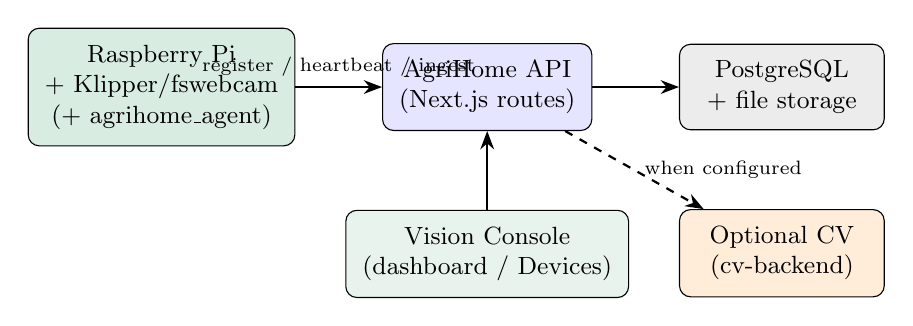
\begin{tikzpicture}[
  font=\small,
  box/.style={draw, rounded corners, align=center, inner sep=6pt, minimum width=2.6cm},
  arr/.style={-{Stealth}, thick}
]
\node[box, fill=leafgreen!20] (pi) {Raspberry Pi\\+ Klipper/fswebcam\\(+ agrihome\_agent)};
\node[box, fill=blue!10, right=1.1cm of pi] (api) {AgriHome API\\(Next.js routes)};
\node[box, fill=gray!15, right=1.1cm of api] (store) {PostgreSQL\\+ file storage};
\node[box, fill=leafgreen!12, below=1.0cm of api] (ui) {Vision Console\\(dashboard / Devices)};
\node[box, fill=orange!15, below=1.0cm of store] (cv) {Optional CV\\(cv-backend)};

\draw[arr] (pi) -- node[above, font=\scriptsize]{register / heartbeat / ingest} (api);
\draw[arr] (api) -- (store);
\draw[arr] (ui) -- (api);
\draw[arr, dashed] (api) -- node[right, font=\scriptsize]{when configured} (cv);
\end{tikzpicture}
\caption{Summer 2026 system overview: Pi+Klipper to AgriHome API to storage/DB and dashboard, with optional CV.}
\label{fig:charter-overview}
\end{figure}

\begin{verbatim}
        +------------------+
        |  Vision Console  |
        |  (Next.js PWA)   |
        +--------+---------+
                 |
                 v
        +----------------------+
        | AgriHome Next.js API |
        | /api/raspberry-pi/*  |
        | /api/devices/* ...   |
        +----------+-----------+
              |           |
              v           v
     +-------------+  +----------------+
     | PostgreSQL  |  | STORAGE_* files |
     | trays/plants|  | /api/files/...  |
     | edge_devices|  +----------------+
     +-------------+
              ^
              |  optional
              v
     +------------------+     +---------------------+
     | cv-backend       |     | Pi + Klipper        |
     | species classify |<--->| agrihome_agent      |
     +------------------+     +---------------------+
\end{verbatim}

\section{Roles \& Responsibilities}
Stakeholders want a compact plant monitor that can detect diseases and reduce constant manual
inspection. The sponsor is Professor Noor.

Key team roles (rotated across sprints as directed by course practice):
\begin{itemize}
  \item \textbf{Scrum master} --- backlog facilitation and sponsor contact; expected to also contribute
        to another technical role.
  \item \textbf{Hardware designers/programmers} --- plant rack, camera fixture, Raspberry Pi /
        Agri-Home/klipper bench setup (fswebcam), and edge agent bring-up.
  \item \textbf{Software programmers} --- Vision Console UI, Next.js API routes, PostgreSQL schema/
        migrations, and Firebase session integration.
  \item \textbf{AI designers} --- \texttt{cv-backend} training/serving, species inference wiring, and
        evaluation of post-capture detection quality.
\end{itemize}

Roles are not permanent for the duration of the project. Members may hold multiple roles. The scrum
master role rotates at the end of each sprint at the request of Professor Noor. Assignments follow
expertise, so people often return to similar task clusters across sprints.

\section{Cost Proposal}
The budget allotted by the customer is \$800, sourced from the CSE department of UTA. Funds cover
image-capture hardware (including Raspberry Pi / webcam components as needed), compute for
running models, materials for the testbed, and incidental implementation costs. University-provided
server capacity continues to offset hosting costs where available.

\subsection{Preliminary Budget}
\begin{table}[H]
\centering
\begin{tabular}{@{}lr@{}}
\toprule
\textbf{Item} & \textbf{Estimated Cost} \\
\midrule
Camera / webcam module & \$70 \\
Computer (local / Pi-class edge) & \$60--\$120 \\
Computer (server) & \$0 (provided by UTA where available) \\
Camera fixture & \$50 \\
Plant fixture / tray materials & \$100 \\
Plants & \$50 \\
Misc.\ networking / mounting & \$50 \\
\bottomrule
\end{tabular}
\caption{Preliminary budget (updated for edge capture components).}
\label{tab:budget}
\end{table}

\subsection{Current \& Pending Support}
The primary funding source is the CSE Department of The University of Texas at Arlington. The
default amount of \$800 should cover projected costs. If additional funding is required, Professor Noor
has indicated willingness to provide support, though no exact amount or formal commitment has been
made.

\section{Facilities \& Equipment}
Most equipment needed is available at UTA. Construction of the plant rack and camera fixture uses
makerspaces (Nedderman Hall and Library), including saws and 3D printers; CNC or laser cutting may
be used if the fixture design requires it.

AI model training and deployment need GPU-capable machines. Senior Design lab computers may
suffice subject to availability; otherwise team machines or containerized \texttt{cv-backend} workflows
are used. External rented GPUs remain a fallback but are not required for the current scope.

Edge integration requires bench networking so (1)~Pi agents can reach the AgriHome API (LAN,
Cloudflare tunnel, or other HTTPS endpoint) and (2)~optional HTTP streamer URLs on \texttt{klipper\_url} are reachable when server-side stills are used
when using the server-side Take Picture fast path (often \texttt{http://PI\_IP:7125} API and/or nginx
\texttt{:80} webcam stills, or a tunnel URL when the host cannot see the Pi LAN). Stable temperature
and electrical supply are required for plant care; the Senior Design lab or Engineering Research
Building balcony spaces remain candidate storage/test sites.

\section{Assumptions}
\begin{itemize}
  \item Sufficient labeled leaf disease images (e.g., PlantVillage-style) remain available for training
        and evaluation of the classifier.
  \item Raspberry Pi + Agri-Home/klipper + \texttt{fswebcam} hardware is available for the Hardware \&
        Software Integration (Pi) sprint.
  \item Team members have consistent access to computing resources for Next.js development,
        PostgreSQL, and model training/serving.
  \item Lab spaces remain available during normal operating hours for setup and testing.
  \item The image recognition model can achieve acceptable classification performance (e.g.,
        $>$80\% validation accuracy) within the planned training period when CV is in scope.
  \item Lighting during capture is sufficiently controlled to avoid extreme image-quality variability.
  \item A shared \texttt{DEVICE\_PROVISIONING\_SECRET} can be distributed securely to bench devices.
  \item Pi agents can reach AgriHome over LAN or via Cloudflare tunnel / public HTTPS; operators
        can set a reachable \texttt{klipper\_url} (LAN IP or tunnel) for optional server-side stills.
  \item Course schedule and instructor expectations remain consistent with the projected sprint
        timeline (CSE~4316 historically; CSE~4317 continuation in Summer 2026).
\end{itemize}

\section{Constraints}
\begin{itemize}
  \item Prototype demonstrations must complete within the senior-design course calendar (Spring /
        Summer 2026 milestones).
  \item Total development costs must not exceed the allocated \$800 budget unless additional sponsor
        funding is approved.
  \item Development follows the sprint schedule defined by the course syllabus.
  \item The system must operate using consumer-grade cameras/webcams and computing hardware
        (including Raspberry Pi-class devices).
  \item The solution must comply with university IT and lab usage policies.
  \item Only publicly available datasets or self-collected images may be used for model training.
  \item Team size and available development hours are fixed by course enrollment and academic
        commitments.
  \item Device registration remains closed unless \texttt{DEVICE\_PROVISIONING\_SECRET} is configured;
        plaintext device API keys are shown only once at register/rotate.
\end{itemize}

\section{Risks}
Risk exposure is calculated as $\mathrm{Exposure} = \mathrm{Probability} \times \mathrm{Loss}$ (in days).

\begin{table}[H]
\centering
\begin{tabular}{@{}p{6.2cm}ccc@{}}
\toprule
\textbf{Risk description} & \textbf{Prob.} & \textbf{Loss} & \textbf{Exposure} \\
\midrule
Insufficient model accuracy for reliable diagnosis & 0.40 & 15 & 6.0 \\
Limited availability of labeled disease images & 0.35 & 12 & 4.2 \\
Hardware malfunction or camera/webcam failure & 0.25 & 8 & 2.0 \\
Unexpected delays in model training or debugging & 0.30 & 10 & 3.0 \\
Team member availability conflicts & 0.30 & 7 & 2.1 \\
Image quality variability causing inconsistent results & 0.35 & 9 & 3.15 \\
Pi unreachable from AgriHome host (NAT / WARP LAN) & 0.30 & 6 & 1.8 \\
Provisioning secret leakage or stolen device API key & 0.20 & 10 & 2.0 \\
\bottomrule
\end{tabular}
\caption{Overview of highest-exposure project risks (Summer 2026 update).}
\label{tab:risks}
\end{table}

Mitigation strategies include early dataset validation, backup hardware planning, incremental model
testing per sprint, primary agent \texttt{fswebcam} capture with optional HTTP streamer fast path, hashed device keys with
revoke/rotate, ingest rate limits, and documented LAN/WARP override guidance for bench networks.

\section{Documentation \& Reporting}
\subsection{Major Documentation Deliverables}
The Project Charter defines project scope, objectives, stakeholders, and high-level risks. It is reviewed
at major milestone checkpoints and updated when scope, schedule, or risk changes occur.

\subsubsection{Project Charter}
Maintained as a controlled document defining vision, scope, objectives, stakeholders, and high-level
risks. Reviewed at the end of major milestones or sprints. Updates occur for significant scope,
stakeholder, or risk adjustments. Major revisions are version-tracked and approved by the team.

\textit{Initial version delivery:} Sprint~1.
\textit{Final version delivery:} Prior to final project submission (this document is Revision~2.1,
Summer~2026 updated release).

\subsubsection{System Requirements Specification}
Living document reflecting agreed functionality and constraints. Formally reviewed at the beginning
and end of each sprint. Updates occur when requirements are approved, modified, or clarified from
customer feedback, sprint reviews, testing, or scope adjustments. Major requirement changes require
team discussion and approval with version tracking.

\subsubsection{Architectural Design Specification}
Describes high-level structure, major components, interfaces, and data flow. Reviewed each sprint;
updated for significant architectural changes (new subsystems, integration approaches). Companion
ADS for the Vision Console layered architecture remains the Spring 2026 design baseline.

\subsubsection{Detailed Design Specification}
Describes internal design of modules, workflows, data structures, and algorithms. Updated throughout
development and reviewed each sprint. The CSE~4317 Summer~2026 DDS reflects the real Next.js /
PostgreSQL / Raspberry Pi implementation rather than earlier fictional schema drafts.

\subsection{Recurring Sprint Items}
\subsubsection{Product Backlog}
Prioritized list of features and technical work (including edge stories AGRI-101--AGRI-110). Refined
continuously; ordered by customer value and risk.

\subsubsection{Sprint Planning}
Team selects backlog items for the sprint capacity, clarifies acceptance criteria, and identifies
dependencies (hardware bench time, CV model availability, networking).

\subsubsection{Sprint Goal}
Single concise objective for the sprint (example Summer 2026: ``Pi registers, heartbeats, and Take
Picture lands a frame in the Console'').

\subsubsection{Sprint Backlog}
Committed tasks for the sprint, owned by individuals, tracked to done.

\subsubsection{Task Breakdown}
Stories decomposed into implementable tasks (API route, migration, UI panel, agent command,
docs).

\subsubsection{Sprint Burn Down Charts}
Progress visualization of remaining work versus time; used in daily coordination.

\subsubsection{Sprint Retrospective}
Process inspection and adaptation; action items carried into the next planning session.

\subsubsection{Individual Status Reports}
Per-member updates for course reporting requirements.

\subsubsection{Engineering Notebooks}
Design decisions, experiments, and test notes (including Klipper/fswebcam capture and optional streamer URL findings and
provisioning runs).

\subsection{Closeout Materials}
\subsubsection{System Prototype}
Working Vision Console with PostgreSQL, Firebase auth, optional CV, and at least one provisioned
Raspberry Pi capture path.

\subsubsection{Project Poster}
CoE Innovation Day poster summarizing problem, approach, edge integration, and results.

\subsubsection{Web Page}
Project summary page for stakeholders and recruitment/demo context.

\subsubsection{Demo Video}
End-to-end walkthrough: register Pi, heartbeat online, Take Picture, view capture, optional CV.

\subsubsection{Source Code}
Monorepo application code, migrations, \texttt{cv-backend}, and reference \texttt{agrihome\_agent} package.

\subsubsection{Source Code Documentation}
Implementation guide, CV pipeline notes, Raspberry Pi/Klipper ops docs (\texttt{RASPBERRY\_PI\_KLIPPER.md}), and edge security notes.

\subsubsection{Hardware Schematics}
Rack/fixture sketches and Pi/Klipper networking notes as applicable.

\subsubsection{CAD Files}
Fixture designs produced in makerspace workflows.

\subsubsection{Installation Scripts}
Environment templates, migration commands, agent register/run instructions.

\subsubsection{User Manual}
Operator guide for Console navigation, Devices page, tray Pi panel, and schedule destinations.

\newpage
\begin{thebibliography}{9}
\bibitem{mohanty2016}
S.~P. Mohanty, D.~P. Hughes, and M.~Salath\'{e}, ``Using deep learning for image-based plant disease
detection,'' \textit{Frontiers in Plant Science}, 2016.

\bibitem{tomato-cnn}
Surveyed CNN architectures (ResNet, VGG, MobileNet, EfficientNet) for tomato leaf disease
detection in the plant-pathology deep learning literature (2018--2024).

\bibitem{unet-leaf}
U-Net / Mask R-CNN leaf segmentation approaches for isolating plant tissue prior to classification.

\bibitem{klipper}
Agri-Home/klipper companion firmware and \texttt{camera-macros/save\_image.sh} (\texttt{fswebcam}), used for AgriHome edge
capture.

\bibitem{srs}
AgriHome, \textit{System Requirements Specification}, CSE~4316 / updated Summer~2026.

\bibitem{ads}
AgriHome, \textit{Architectural Design Specification}, CSE~4316, Spring~2026.

\bibitem{nextjs}
Vercel, Inc., ``Next.js Documentation,'' \url{https://nextjs.org/docs}.
\end{thebibliography}

\end{document}
